The volumetric power density of high-frequency resonant converters is fundamentally constrained by the thermal limits of the magnetic components. In high-power applications, the transformer is subjected to substantial high-frequency copper and core losses. This chapter details the fundamental design principles and analytical models employed to propose and size the proposed transformer without compromising its electromagnetic performance.

\section{Proposed Transformer Design}
In high-power-density CLLC resonant converters, managing the thermal stresses caused by high-frequency core and winding losses is a critical design constraint. As introduced in Section \ref{sec:cooling}, conventional solutions have a high dependence on active cooling systems to manage these thermal loads. This solution proposes to improve intrinsic thermal extraction from the heat-generating elements, which comprise the windings and the ferrite core, to the external ambient environment. With this solution, the dependence on active cooling methods has a potential to be reduced. 

Therefore, the proposed transformer is fundamentally engineered to improve this heat conduction by maximizing the core window utilization, and minimizing the internal-to-external thermal resistance. To facilitate this, a planar structure utilizing a low-loss Mn-Zn ferrite EE-core is proposed. 

Within this planar structure, the winding configuration is the primary determining factor for heat flow. There are two main configurations for rectangular windings in transformers. Conventionally, planar transformers typically utilize edgewise windings, where the rectangular conductor is wound on its narrow edge, along the vertical axis of the core. To address the inherent bottlenecks of the conventional winding structure, the proposed transformer utilizes solid rectangular windings arranged in a flatwise orientation. This entails that the winding is wound on its broad, flat side, resembling a radial stack propagating from the center.

The proposed structure utilizing a flatwise-wound configuration is shown in Figure \ref{fig:flatwise_3D_trans}. The cross-section of this design is shown in Figure \ref{fig:flatwise_2D_trans}. To ensure optimal thermal contact and maximize heat extraction toward the widest cooling area, a soft, silicon-based thermal-interface material (TIM) is sandwiched directly between the copper windings and the ferrite core interface.

\begin{figure}[h!]
    \centering
    \subfloat[]{
        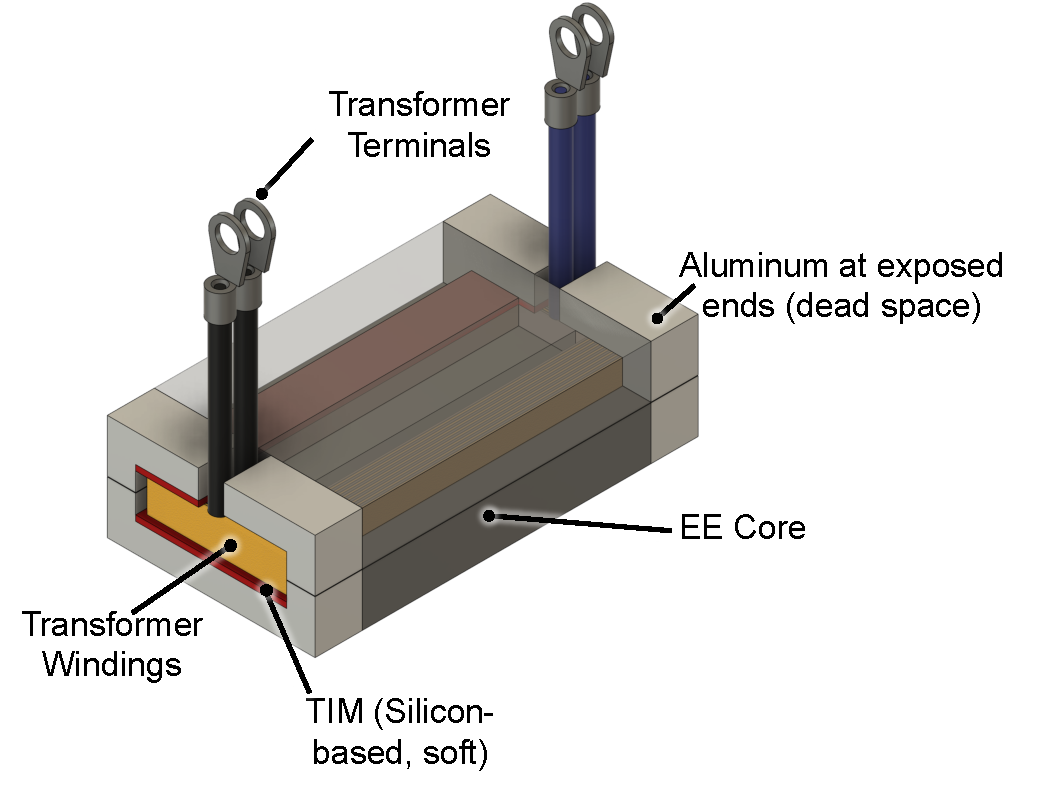
\includegraphics[width=0.5\columnwidth]{figures_chapter3/flatwise_3D.pdf}%
        \label{fig:flatwise_3D_trans}
    }
    \subfloat[]{
        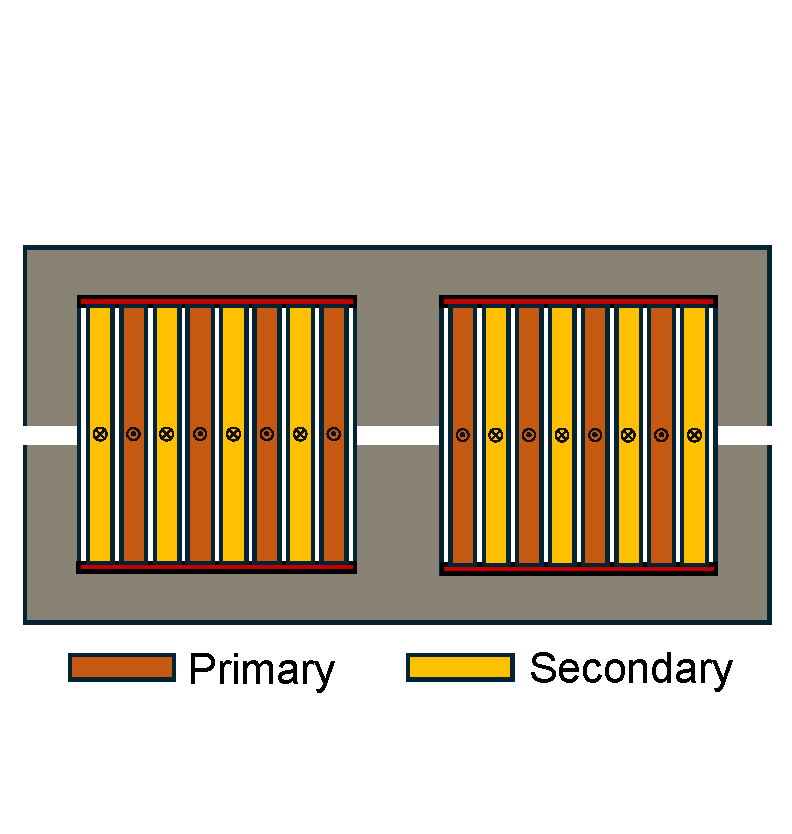
\includegraphics[width=0.3\columnwidth]{figures_chapter3/flatwise_cross.pdf}
        \label{fig:flatwise_2D_trans}
    }
    \caption{Representative model of an flatwise-wound transformer: (a) mockup of the transformer, with the top half of the EE core transparent, and (b) cross-sectional view of the transformer.}
    \label{fig:flatwise_design}
\end{figure}

In the subsequent chapters, this proposed flatwise structure will be rigorously compared against its conventional counterpart through both 3D FEA simulations and empirical hardware testing. The counterpart transformer employs an identical core and TIM structure, but utilizes a traditional edgewise-wound configuration, as shown in Figure \ref{fig:edgewise_3D_trans} and Figure \ref{fig:edgewise_2D_trans} respectively.

\begin{figure}[h!]
    \centering
    \subfloat[]{
        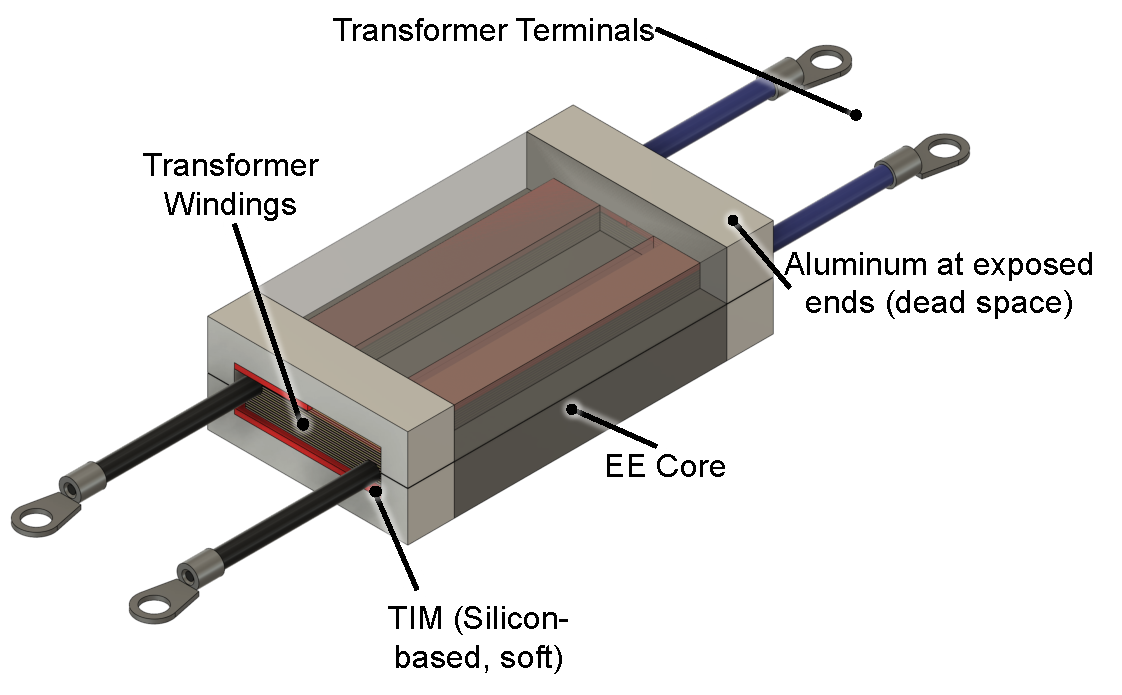
\includegraphics[width=0.5\columnwidth]{figures_chapter3/edgewise_3D.pdf}%
        \label{fig:edgewise_3D_trans}
    }
    \subfloat[]{
        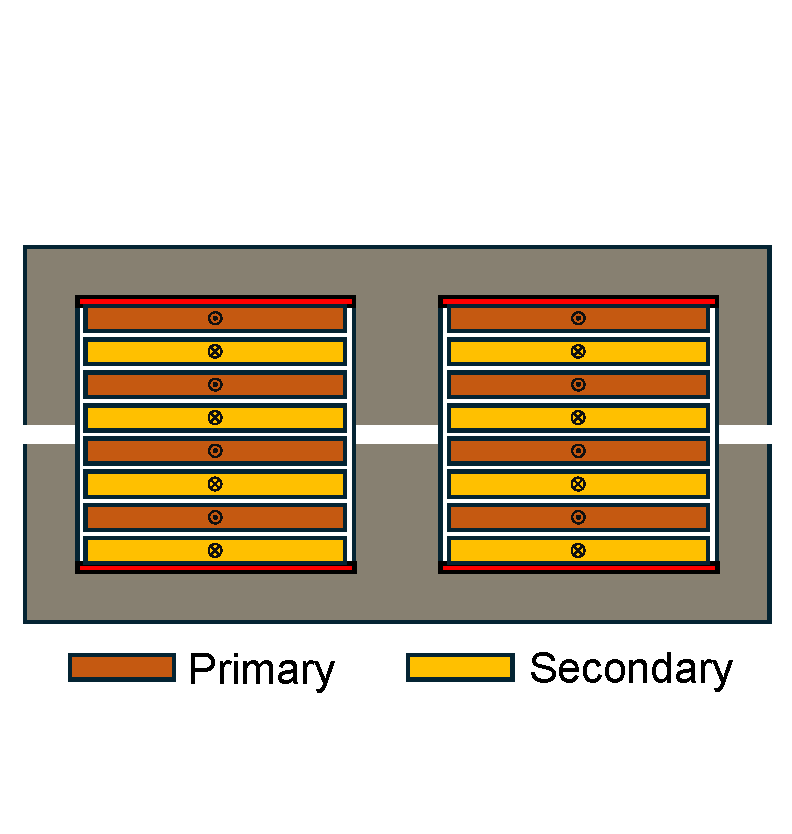
\includegraphics[width=0.3\columnwidth]{figures_chapter3/edgewise_cross.pdf}
        \label{fig:edgewise_2D_trans}
    }
    \caption{Representative model of an edgewise-wound transformer: (a) mockup of the transformer, with the top half of the EE core transparent, and (b) cross-sectional view of the transformer.}
    \label{fig:edgewise_design}
\end{figure}

\subsection{Heat Dissipation Mechanism}\label{section:heat_dissipation}

This section details the mechanism of heat extraction from the windings to the environment depending on the configuration. The design presented regardless of the winding configuration operates on the following principle. The primary thermal dissipation path through the windings is augmented by two supplementary mechanisms, as illustrated in Figure \ref{fig:heatdissipation}. First, the high fill factor enables heat to conduct directly from the copper through a thermal interface material (TIM) into the ferrite core, which functions as a heat spreader. Second, the exposed winding overhangs occupy the volume outside the EE-core, referred to as 'dead space'. This volume is leveraged by attaching aluminum blocks to the top and bottom surfaces of the exposed windings, creating an additional direct path for heat extraction. The heat flow from the lower winding section into the cooling block under external cooling conditions is also illustrated. The substantial surface area of this planar structure facilitates efficient heat transfer to external systems, such as liquid cold plates, which is essential for high-power density applications.

\begin{figure}[h!]
    \centering
    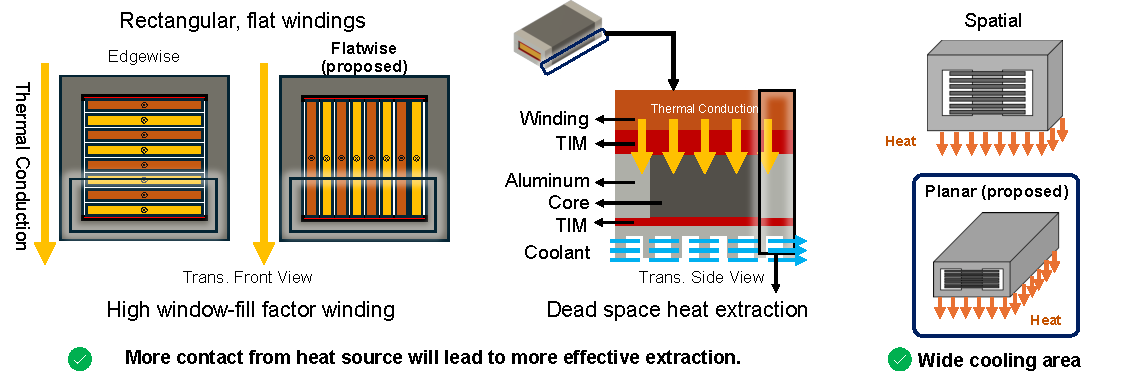
\includegraphics[width=\columnwidth]{figures_chapter3/heatdissipation.pdf}
    \caption{Heat conduction paths for the transformers, with a primary heat transfer path through the windings and supplementary path through an aluminum block in the ‘dead space’, with an external cooling system. The wide surface area for cooling aids in heat dissipation from the transformer.}
    \label{fig:heatdissipation}
\end{figure}

The advantage of the proposed structure compared to its conventional counterpart will be explained once the thermal models are established for each configuration.

\subsection{Winding Configuration}

While optimizing the thermal dissipation path is critical, minimizing internal heat generation is equally important. In high-frequency transformers, winding interleaving is a proven strategy to reduce the peak magnetomotive force (MMF), thereby mitigating AC copper losses driven by skin and proximity effects. To determine the optimal balance of performance and manufacturability for the proposed transformer, this study evaluates three winding configurations: non-interleaved, Primary-Secondary-Secondary-Primary (PSSP) \cite{ref21}, and fully interleaved. A comparison of their extracted parasitic parameters is presented in Table \ref{tab:parasitics}, while their physical implementation is illustrated in Figure~\ref{fig:implementation}.

\begin{table}[h]
    \caption{Comparison of Parasitic Parameters}
    \centering
    
        \begin{tabular}{cccccc}
            \hline
            \textbf{Parameter} & \textbf{Symbol} & \textbf{Non-Inter.} & \textbf{PSSP Inter.} & \textbf{Full Inter.} & \textbf{Unit} \\
            \hline \hline
            AC Res. & $R_{\mathrm{AC}}$ & 40.05 & 21.45 & 21.56 & m$\Omega$ \\
            Interwinding Cap. & $C_{\mathrm{ps}}$ & 0.15 & 0.96 & 1.72 & nF \\
            Leakage Ind. & $L_{\mathrm{lk}}$ & 2.63 & 0.07 & 0.04 & $\upmu$H \\
            \hline
        \end{tabular}%
    
    \label{tab:parasitics}
\end{table}

\begin{figure}[h]
    \centering
    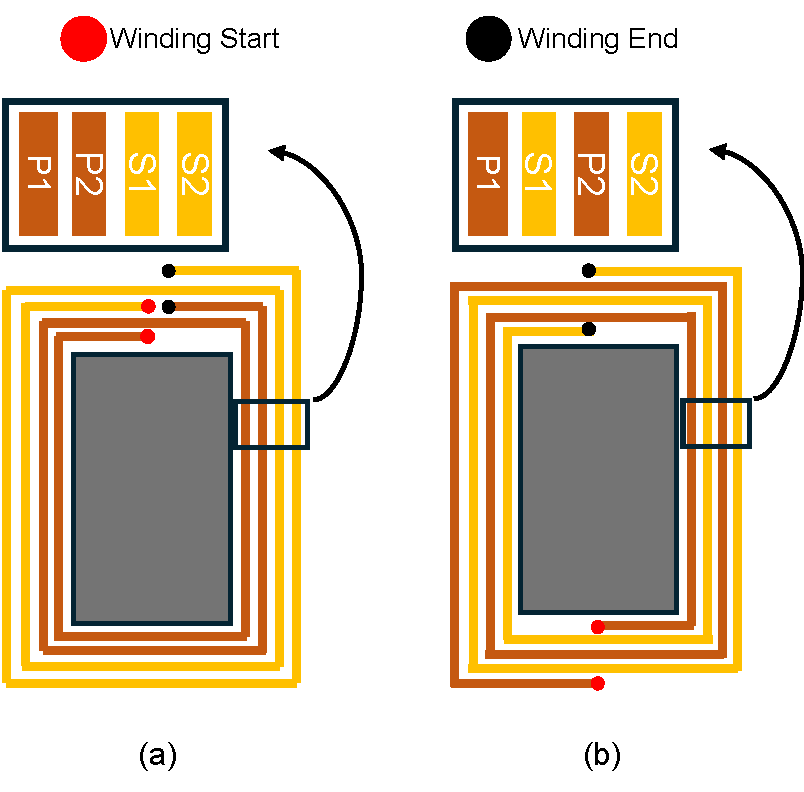
\includegraphics[width=0.5\columnwidth]{figures_chapter3/interleaving implementation.pdf}
    \caption{Schematic representation of the implementation of the interleaving strategies discussed (top view): (a) no interleaving, and (b) full interleaving. Four turns are shown for easy interpretation.}
    \label{fig:implementation}
    
\end{figure}

The selection of the winding arrangement requires balancing leakage inductance, parasitic capacitance, and manufacturability. The fully interleaved model demonstrates the lowest leakage inductance (0.04 $\upmu\text{H}$), a substantial improvement over the non-interleaved baseline (2.63 $\upmu\text{H}$). While this configuration increases the interwinding capacitance to 1.72 nF due to the larger effective overlap area, circuit simulations verify that this capacitance level does not hinder the ZVS operation of the CLLC converter. Conversely, while the non-interleaved model offers minimal capacitance (0.15 $\text{nF}$), the associated high leakage inductance and AC resistance result in prohibitive losses for this high-power density application.

The PSSP configuration presents an intermediate trade-off, offering reduced AC resistance (21.45 $\text{m}\Omega$) with moderate capacitance. However, PSSP interleaving introduces significant manufacturability constraints. Moreover, as this was examined in a discrete turn case, then once the winding becomes continuous, it would not be implementable.

Therefore, the fully interleaved configuration is selected. It provides the optimal balance by minimizing AC losses and maintaining circuit stability.

\section{Transformer Modelling}

\subsection{Geometric Model}
To establish a lot of the terms to be used in the subsequent sections, a geometric model is first defined. To simplify the analysis, the windings will be treated as discrete layers per turn. A parametric geometric model is created for the flatwise-wound transformer based on the winding dimensions ($w_{\mathrm{wire}}$, $h_{\mathrm{wire}}$), number of turns ($N_{\mathrm{p}}$), and the inter-winding distance ($d_{\mathrm{inter}}$), allotted for isolation. An air gap $l_\mathrm{g}$ is also included. The TIM thickness ($d_{\mathrm{TIM}}$) and core clearances ($d_{\mathrm{clear}}$) are also considered in determining the final core dimensions. A similar model is also derived for the edgewise-wound transformer. The models for the edgewise-wound and flatwise-wound transformers are shown in Figure~\ref{fig:edgewise_parameter} and \ref{fig:flatwise_parameter} respectively. This flow of modelling is inspired by \cite{bahmani2016design}.

\begin{figure}[h!]
    \centering
    \subfloat[]{
        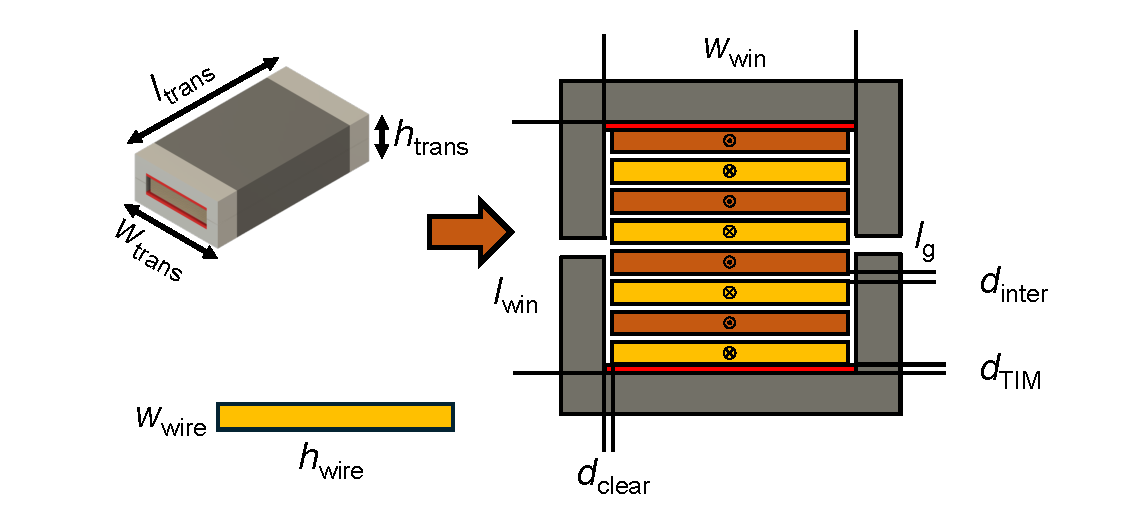
\includegraphics[width=0.85\columnwidth]{figures_chapter3/edgewise_parameter.pdf}%
        \label{fig:edgewise_parameter}
    }

    \subfloat[]{
        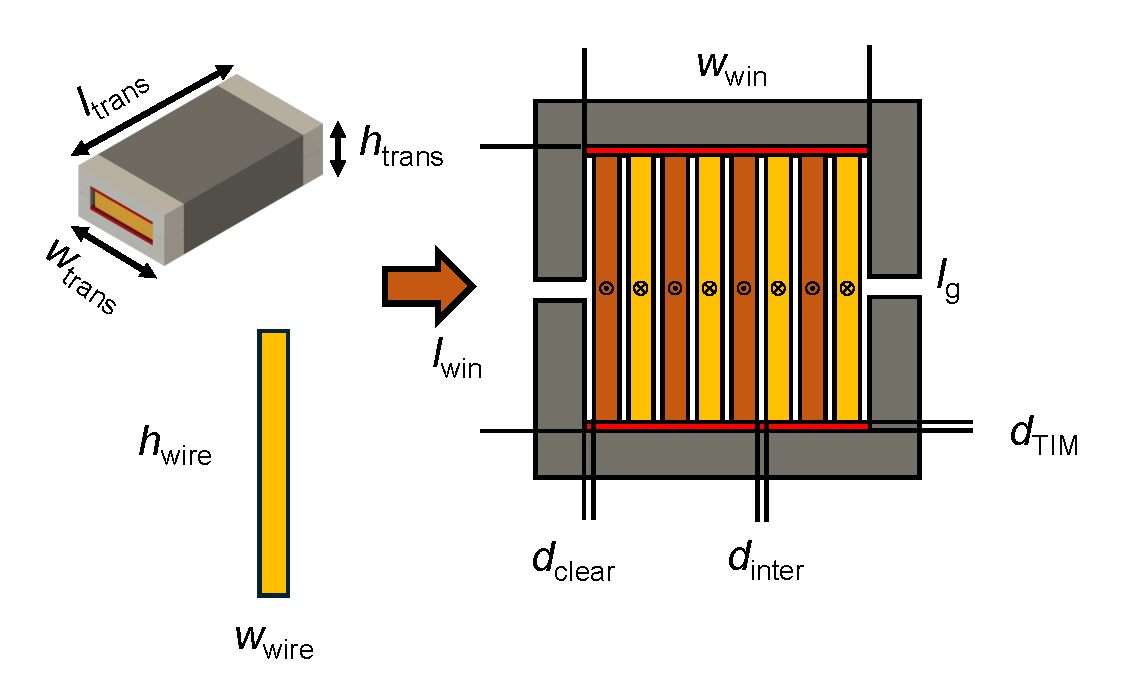
\includegraphics[width=0.8\columnwidth]{figures_chapter3/flatwise_parameter.pdf}
        \label{fig:flatwise_parameter}
    }
    \caption{Parametric model of an (a) edgewise-wound transformer (conventional) and (b) flatwise-wound transformer (proposed).}
    \label{fig:parameteric models}
\end{figure}

The core window dimensions are important to obtain other geometric parameters of the transformer. The window height $h_{\mathrm{win}}$ and width $w_{\mathrm{win}}$ can be obtained with the following as shown in Eq.~\ref{eq:hwin} and Eq.~\ref{eq:wwin} respectively for the flatwise-wound transformer. 
\begin{align}
    h_{\mathrm{win}} &= h_{\mathrm{wire}} + 2 d_{\mathrm{TIM}} \label{eq:hwin} \\
    w_{\mathrm{win}} &= 2N_{\mathrm{p}} w_{\mathrm{wire}} + (2N_{\mathrm{p}} - 1) d_{\mathrm{inter}} + 2 d_{\mathrm{clear}} \label{eq:wwin}
\end{align}

For the conventional counterpart, the equations look similar, with Eq. ~\ref{eq:hwinedge} and Eq. ~\ref{eq:wwinedge} representing the window height and width respectively. 
\begin{align}
    h_{\mathrm{win}} &= 2N_{\mathrm{p}} w_{\mathrm{wire}} + (2N_{\mathrm{p}} - 1) d_{\mathrm{inter}} + 2 d_{\mathrm{TIM}} \label{eq:hwinedge}\\
    w_{\mathrm{win}} &= h_{\mathrm{wire}} + 2 d_{\mathrm{clear}} \label{eq:wwinedge}
\end{align}
A few more quantities can be obtained after looking at the transformer from the top. From Figure \ref{fig:core_top}, $l_\mathrm{core}$ and $w_\mathrm{core}$ represent the length and width of the center leg respectively. As per commercial standard, the width of the outer leg is half of $w_\mathrm{core}$. 

\begin{figure}[h!]
    \centering
    \subfloat[]{
        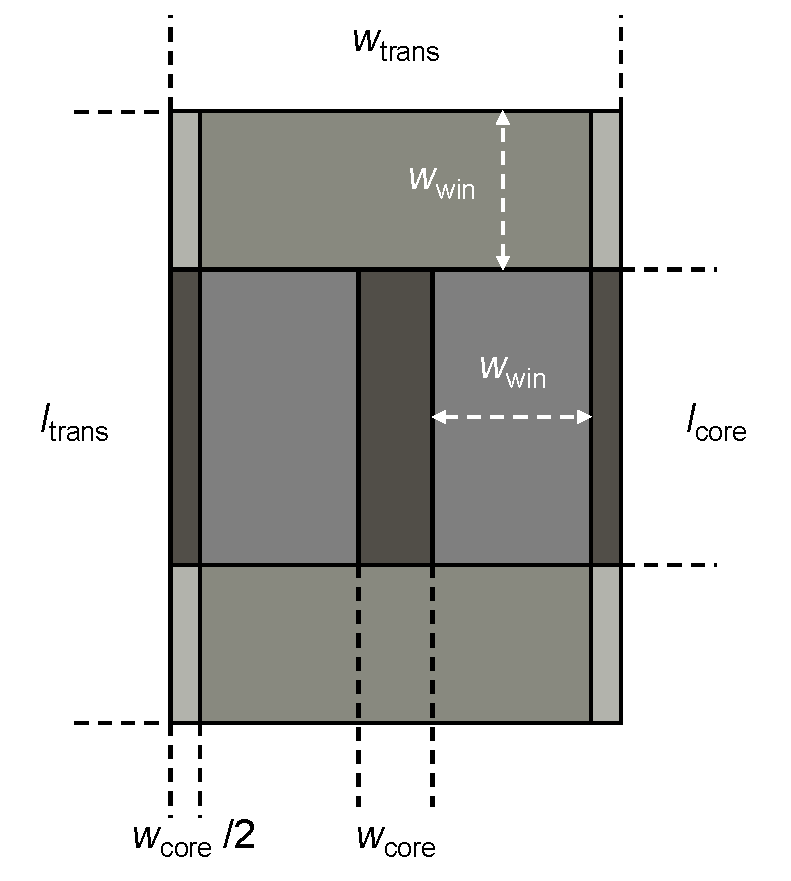
\includegraphics[width=0.5\columnwidth]{figures_chapter3/core_top.pdf}%
        \label{fig:core_top}
    }

    \subfloat[]{
        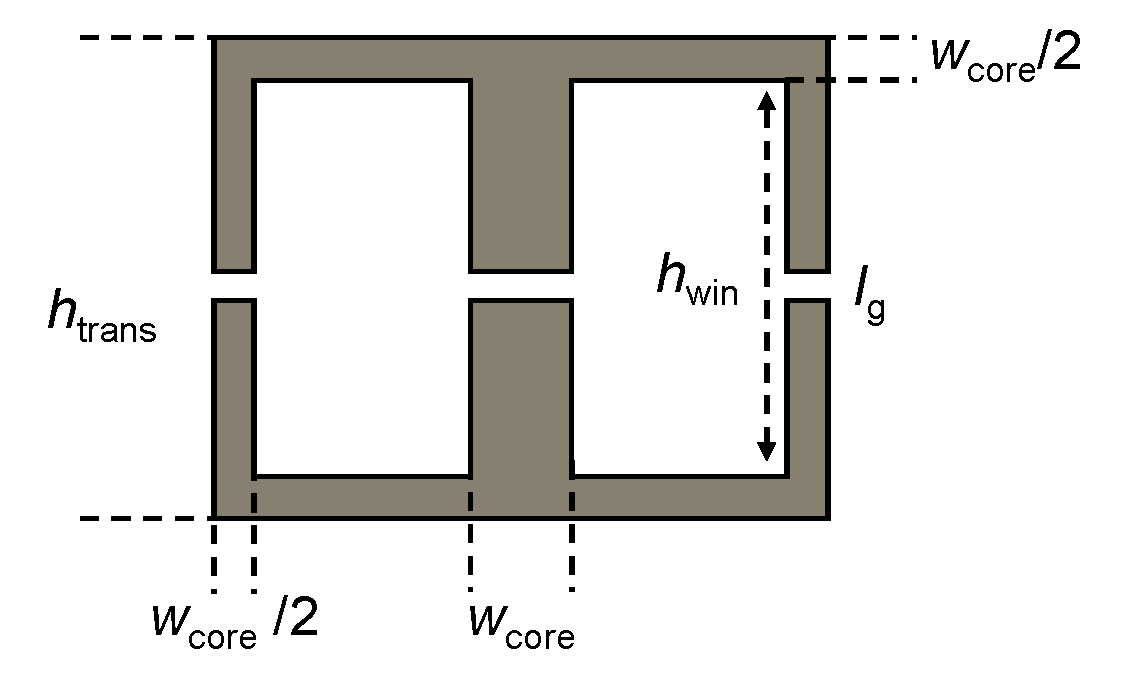
\includegraphics[width=0.5\columnwidth]{figures_chapter3/core_front.pdf}
        \label{fig:core_front}
    }
    \caption{(a) Top view and (b) Front view of the transformer geometric model.}
    \label{fig:parameteric models core}
\end{figure}

The transformer dimensions are obtained by using Eq.~\ref{eq:ltrans} --~\ref{eq:htrans}. Moreover, the aluminum block for dead space has a length of $w_{\mathrm{win}}$ regardless of the winding configuration. The TIM is applied throughout the top and bottom of the core window with width $w_{\mathrm{win}}$, ensuring maximum contact between the windings and the heat spreader. The box dimensions are represented in Figure \ref{fig:parameteric models}.
\begin{align}
    l_{\mathrm{trans}} &= l_{\mathrm{core}} + 2w_{\mathrm{win}}  \label{eq:ltrans}\\
    w_{\mathrm{trans}} &= w_{\mathrm{core}} + 2 w_{\mathrm{win}} + 2 \cdot \frac{w_\mathrm{core}}{2} \label{eq:wtrans}\\
    h_{\mathrm{trans}} &= 2 \cdot \frac{w_\mathrm{core}}{2} + h_{\mathrm{win}}\label{eq:htrans} 
\end{align}


Lastly, the mean turn length (MTL) of each of the configurations can be denoted by Eq. ~\ref{eq:MTL}. A simpler analogy to denote this is that the mean turn length is the length of the turn halfway through the core window. 
\begin{align}
    \mathrm{MTL} &= 2l_{\mathrm{core}} + 2w_{\mathrm{core}} + 8w_{\mathrm{win}} \label{eq:MTL} 
\end{align}

\subsection{Thermal Modeling}
To evaluate the fundamental heat dissipation mechanisms of the conventional edgewise and proposed flatwise winding configurations, analytical 1D Thermal Networks are constructed, as they are highly effective and widely adopted for planar magnetics \cite{ref13}, \cite{escribano2006new}, \cite{lewaiter2001thermal}, \cite{vanderlinde1991design}, \cite{chen2002volumetric}. Because the primary external cooling boundaries (the TIM and core) are located at the top and bottom of the winding window, the dominant conductive heat flux is strictly unidirectional (vertical). Therefore, lateral (side-to-side) heat transfer across the winding window can be mathematically neglected, allowing a simplified 1D thermal resistance network to accurately capture the primary heat extraction path.

In a thermal model, each loss source is modeled as a discrete current source. For a transformer, this includes the winding loss and core loss. The winding loss is separated per turn, denoted as $P_{\mathrm{Np1}}\, , P_{\mathrm{Ns1}}\, , \dots \, , P_{\mathrm{Npn}}\, , P_{\mathrm{Nsn}}$ while the core loss is defined as $P_{\mathrm{core}}$. Moreover, to extract heat away from the transformer towards the ambient $T_\mathrm{amb}$, radiation $R_\mathrm{rad}$ and convection $R_\mathrm{conv}$ are taken into account and are placed towards the end of the network, at both sides. Additional thermal resistances are added depending on the cooling method. But for the purposes of explaining the concept, these are not added yet.

A comparative representation of the heat flow towards the cooling boundaries must be analyzed through the fundamental equation for conductive thermal resistance:
\begin{equation}
R_{\mathrm{th}} = \frac{d}{k \cdot A}
\label{eq:Rth}
\end{equation}
where $d$ is the conduction path length, $k$ is the thermal conductivity of the material, and $A$ is the cross-sectional heat transfer area. 

It is important to note that the models that will be presented here are for the purpose of explaining the proposed concept. 3D FEA will be used to provide accurate thermal mapping and visualization. 

A common design concern when comparing the flatwise and edgewise structures is the apparently restricted heat extraction area of the flatwise configuration. In the flatwise winding, the surface area of each individual turn directly facing the primary cooling boundary (the TIM and core) is indeed limited to the narrow, thin edge of the rectangular conductor. Conversely, the conventional edgewise configuration places the wide, broad side of the top and bottom turns directly in contact with the cooling plane. 
To calculate the true physical heat transfer area, the 2D cross-sectional contact width must be multiplied by the orthogonal depth of the winding trace going into the core window $l_{\mathrm{depth}}$. In this analysis, a rectangular section of the core is considered, with width $w_\mathrm{win}$ and length $l_\mathrm{depth}$. Furthermore, because the flatwise turns are positioned side-by-side, the total available window width $w_{\mathrm{win}}$ must be shared between the copper edges and the inter-turn dielectric insulation $d_{\mathrm{inter}}$. The total physical copper contact area for the flatwise configuration is defined as:
\begin{equation}
A_{\mathrm{contact, flat}} = l_{\mathrm{depth}} \cdot \sum_{i=1}^{N} w_{\mathrm{wire}, i} = l_{\mathrm{depth}} \cdot \left( w_{\mathrm{win}} - \sum_{j=1}^{N-1} d_{\mathrm{inter}, j} - 2 d_\mathrm{clear}\right)
\end{equation}

Conversely, the conventional edgewise configuration places the broad side of the top and bottom turns directly in contact with the cooling plane. The total copper contact area is therefore:
\begin{equation}
A_{\mathrm{contact, edge}} = l_{\mathrm{depth}} \cdot h_{\mathrm{wire}} = l_{\mathrm{depth}} \cdot \left(w_\mathrm{win} - 2d_\mathrm{clear}\right)
\end{equation}

Therefore, the flatwise configuration mathematically presents a smaller physical copper contact area to the external TIM ($A_{\mathrm{contact, flat}} < A_{\mathrm{contact, edge}}$) due to the spatial penalty of the vertical insulation strips.

The critical divergence that overcomes this area reduction lies in the network topology and the extreme discrepancy between the thermal conductivities of copper ($k_{\mathrm{Cu}} \approx 400 \text{ W/(m}\cdot\text{K)}$) and dielectric insulation materials ($k_{\mathrm{ins}} \approx 0.1 \text{ to } 0.2 \text{ W/(m}\cdot\text{K)}$).

\subsubsection{Edgewise-wound Transformer Thermal Model}
In the conventional edgewise configuration, the windings are stacked vertically, creating a series thermal path. Because the turns are stacked on top of one another, the heat generated in the innermost turns (e.g., Turn $N/2$) must conduct vertically through multiple layers of copper and, crucially, multiple layers of inter-turn insulation to reach the external cooling boundary.  Here, $N = 2N_\mathrm{p}$. A simple illustration of the heat flow from the windings to the core is shown in Figure \ref{fig:edgewise_heat}. 

\begin{figure}[h!]
    \centering
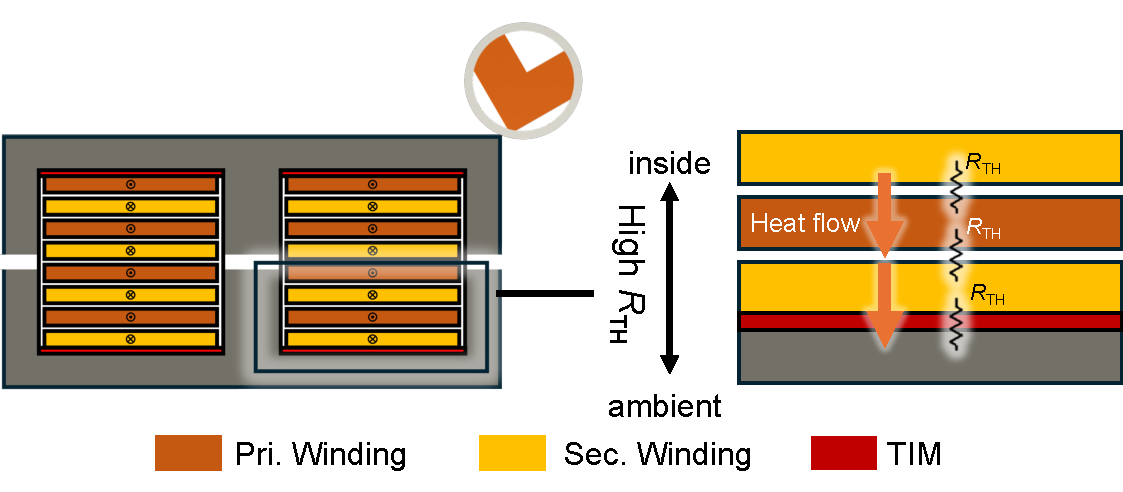
\includegraphics[width=0.8\columnwidth]{figures_chapter3/edgewise_heat.pdf} 
\caption{Simple representation of the edgewise-wound (conventional) transformer, with the cross-sectional area of the transformer. The heat flow direction
is also illustrated through a close-up.} \label{fig:edgewise_heat}
\end{figure}

Even though the heat transfer area $A_{\mathrm{contact, edge}}$ is large, it is severely obstructed by the series addition of multiple insulation thermal resistances ($R_{\mathrm{ins}}$). Because $k_{\mathrm{ins}}$ is approximately 2000 to 4000 times lower than $k_{\mathrm{Cu}}$, even a sub-millimeter layer of dielectric insulation acts as an immense thermal wall.

The thermal model for the edgewise-wound transformer is shown in Figure \ref{fig:edgewise_thermalmodel}. The total internal thermal resistance of the edgewise stack from the center to the cooling boundary is expressed as shown in Equation \ref{eq:edgewise_rth}. 
\begin{equation}
R_{\mathrm{th, edgewise}_\mathrm{total}} = \frac{N}{2} \left( \frac{w_{\mathrm{wire}}}{k_{\mathrm{Cu}} \cdot h_{\mathrm{wire}} \cdot l_\mathrm{depth}} + \frac{d_{\mathrm{inter}}}{k_{\mathrm{ins}} \cdot h_{\mathrm{wire}} \cdot l_\mathrm{depth}} \right) \label{eq:edgewise_rth}
\end{equation}
As $N$ scales, the summation of the high-resistance insulation terms dominates the network, trapping heat in the center turns. 
\begin{figure}[h!]
    \centering
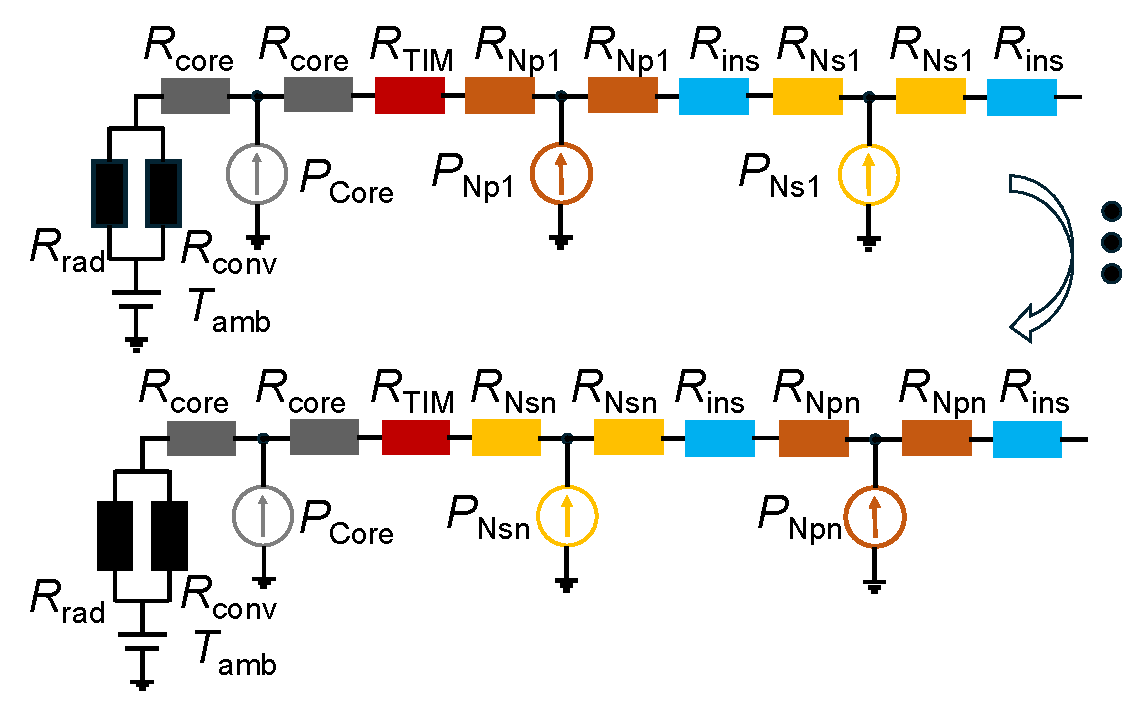
\includegraphics[width=0.8\columnwidth]{figures_chapter3/edgewise_thermalpath.pdf}
\caption{Thermal model for the edgewise-wound (conventional) transformer.}\label{fig:edgewise_thermalmodel}
\end{figure}
\subsubsection{Flatwise-wound Transformer Thermal Model}
In the proposed flatwise configuration, the turns are wound flat and propagate radially outward. This configuration transforms the series thermal trap into a highly efficient parallel thermal path. A simple illustration of the heat flow from the windings to the core is shown in Figure \ref{fig:flatwise_heat}. 
\begin{figure}
    \centering
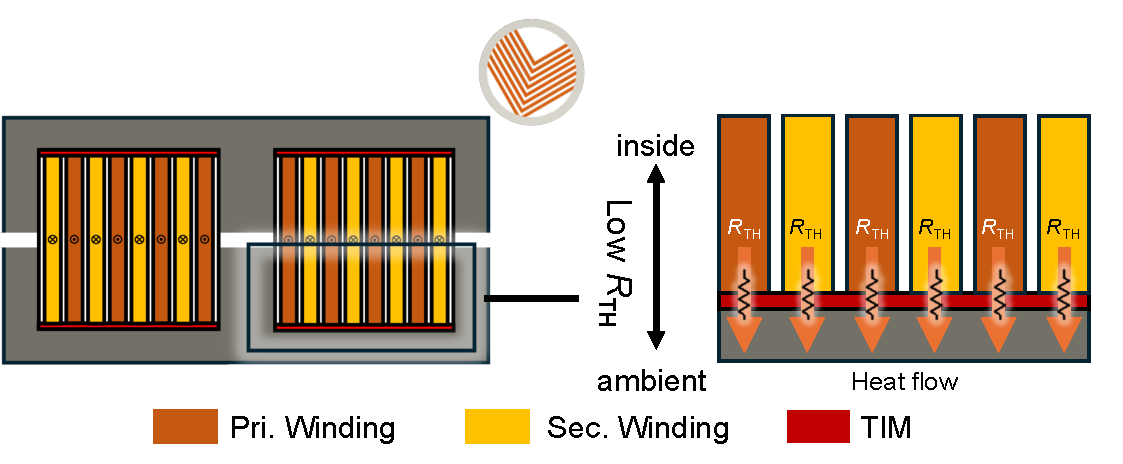
\includegraphics[width=0.8\columnwidth]{figures_chapter3/flatwise_heat.pdf}
\caption{Simple representation of the flatwise-wound (proposed) transformer, with the cross-sectional area of the transformer. The heat flow direction
is also illustrated through a close-up.}\label{fig:flatwise_heat}
\end{figure}

Because the turns are positioned side-by-side, every single individual turn maintains direct, independent contact with the top and bottom TIM and cooling boundaries via its narrow edge. To escape, the heat generated inside any given turn only needs to travel vertically through its own solid copper body to its exposed edge. It does not cross a single inter-turn dielectric insulation barrier ($d_{\mathrm{inter}}$) in series. The parallel thermal resistance of the flatwise winding is defined as shown in Eq. \ref{eq:flatwise_rth}. Here, $N = 2N_\mathrm{p}$.
\begin{equation}
R_{\mathrm{th, flatwise_\mathrm{total}}} = \frac{1}{\left(N\cdot  \frac{h_{\mathrm{wire}}/2}{k_{\mathrm{Cu}} \cdot w_{\mathrm{wire}}\cdot l_\mathrm{depth}} \right)^{-1}}\label{eq:flatwise_rth}
\end{equation}

Although the physical contact area per turn is restricted to $h_{\mathrm{wire}}$, the heat conduction path is entirely within solid copper. Because copper is an exceptionally efficient thermal conductor, the low resistance of the continuous copper path easily compensates for the reduced contact area. 

\begin{figure}
    \centering
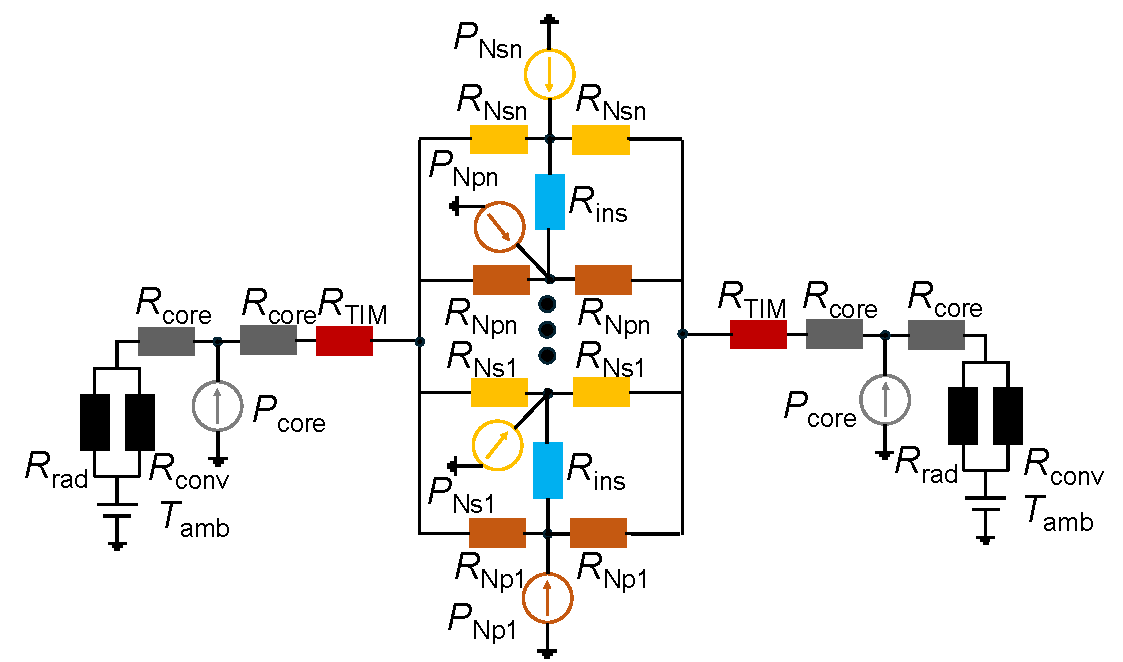
\includegraphics[width=0.8\columnwidth]{figures_chapter3/flatwise_thermalpath.pdf}
\caption{Thermal model for the edgewise-wound (conventional) transformer.}\label{fig:flatwise_thermalmodel}
\end{figure}

 By utilizing a low-resistance parallel copper path in the flatwise design, the proposed transformer fundamentally eliminates internal thermal barriers, enabling highly efficient, simultaneous uniform heat extraction directly from the windings to the core window. It is expected that a more uniform distribution of temperature will be seen throughout the transformer.


%The efficiency of this internal heat dissipation can be explicitly examined through the use of thermal models. A thermal model translates the physical geometry into an equivalent network of thermal resistances to evaluate conductive heat transfer from the internal layers to the ambient environment. For this study, 1D-Thermal Models are constructed. With planar magnetics, the dominant heat extraction path remains to be the surfaces.

%While 3D Finite Element Analysis (FEA) provides comprehensive spatial mapping, analytical 1D lumped-parameter thermal networks are highly effective and widely adopted for planar magnetics \cite{ref15, bahmani2016}. As established in recent planar thermal reviews, the inherent high surface-area-to-volume ratio of flat magnetic structures results in a dominant conductive heat flux that is strictly orthogonal. Therefore, transverse and longitudinal heat transfer can be mathematically neglected, allowing a 1D thermal resistance model to accurately capture the primary path of least thermal resistance.

%In a thermal model, each loss source is modeled as a discrete current source. For a transformer, this includes the winding loss and core loss. The winding loss is separated per turn, denoted as $N_p1, ..., N_pn$. Moreover, to extract heat away from the transformer, radiation and convection are taken into account and are placed towards the end of the network, at both sides. Additional thermal resistances are added depending on the cooling method. But for the purposes of explaining the concept, these are not added yet. Additionally, the thermal resistance of an element $R_{\mathrm{th}}$ is defined as follows:


%The conventional edgewise configuration creates a high-resistance series thermal path that tends to trap heat in the central layers. The corresponding thermal model of the edgewise-wound transformer is shown in Figure xx, derived using the principles from [13].

%In contrast, the proposed flatwise configuration creates a parallel thermal path from winding to core, enabling direct and simultaneous heat extraction from each individual turn. This results in a significantly lower overall internal thermal resistance compared to the conventional counterpart. The thermal model of the flatwise-wound transformer is shown in Figure xx. This then entails a more even heat distribution and lower peak temperature.

%From here on out, a simplified transformer model will be used to examine and easily optimize the dimensions. Each turn will be treated as a discrete turn, stacked from top to bottom for the edgewise-wound transformer, and from center to outward for the flatwise wound transformer, both wound at the center leg.

%In contrast, the proposed flatwise configuration creates a parallel thermal path from winding to core, enabling direct and simultaneous heat extraction from each individual turn. This results in a significantly lower overall internal thermal resistance compared to the conventional counterpart. The thermal model of the flatwise-wound transformer is shown in Figure \ref{fig:fig3b}. This then entails a more even heat distribution and lower peak temperature.

%In the subsequent sections, a simplified transformer model will be used to examine and easily optimize the dimensions. 

\subsection{Isolation Distance}
As mentioned in Section \ref{sec:challenge}, isolation is required to be able to cater to higher voltage applications. It is not yet a current focus of the study. However, ensuring that the transformer is able to cater to basic capabilities is important. It is set as a basic constraint for the transformer, as it essentially affects the overall geometry depending on the number of turns. Moreover, because the windings are rectangular, then the electric field distribution between each primary and secondary turn can be approximated to be the same as that of a parallel-plate capacitor \cite{bahmani2016design}.

Because the windings are rectangular, the windings can be approximated as plate capacitors. Therefore, the minimum isolation distance $d_{\mathrm{inter, min}}$ can be defined as in Eq. \ref{eq:iso, min}.
\begin{align}
d_\mathrm{inter, min} = \frac{V_\mathrm{ins}}{k_\mathrm{saf}E_\mathrm{ins}}\label{eq:iso, min}
\end{align}
\noindent where $V_\mathrm{ins}$ is the expected voltage requirement, and $E_\mathrm{ins}$ is the dielectric material breakdown strength. A safety factor $k_{\mathrm{saf}}$ is also included. 

For the minimum clearance between the windings and the core, $d_{\mathrm{clear, min}}$, it is assumed that the core will be grounded in higher power applications \cite{bahmani2016design}. Therefore, $d_{\mathrm{clear, min}}$ can be estimated with the operating voltage $V_{\mathrm{in}}$, as shown in Eq. \ref{eq:clear, min}. The same equation can be used to estimate the minimum thickness of the TIM, $d_\mathrm{TIM, min}$.
\begin{align}
d_\mathrm{clear, min} = d_\mathrm{TIM, min} = \frac{V_\mathrm{in}}{k_\mathrm{saf}E_\mathrm{ins}}\label{eq:clear, min}
\end{align}

The distance is calculated first and then further confirmed in FEM if it suits the criteria. This is explained further in the next chapter, section \ref{sec:breakdown}.

\subsection{Magnetic Circuit}
A baseline magnetic circuit model is established to evaluate the magnetization properties of the transformer, as indicated in Figure \ref{fig:mag}. The outer leg and core leg magnetic reluctances are denoted as $\mathcal{R}_\mathrm{mo}$ and $\mathcal{R}_\mathrm{mc}$ respectively. The gap reluctances in the outer and center legs are denoted as $\mathcal{R}_\mathrm{go}$ and $\mathcal{R}_\mathrm{gc}$ respectively. 

For this analytical derivation, the transformer is initially assumed to have ideal magnetic coupling, as further strengthened by the full interleaving strategy employed in this transformer. This is assumed to decouple the resonant tank design from the thermal evaluation of the winding structure. Instead, discrete resonant inductors are employed for the resonant tank of the converter.  The secondary side is deactivated (open-circuited) to isolate the primary magnetizing flux, which yields the fundamental expression for the primary magnetizing inductance as shown in Eq. \ref{eq:Lm}:
\begin{equation}
L_\mathrm{m} = \frac{N_\mathrm{p}^2}{\mathcal{R}_{\mathrm{m, eq}}}\label{eq:Lm}
\end{equation}
where $N_p$ is the primary number of turns and $\mathcal{R}_\mathrm{m, eq}$ is the total equivalent reluctance of the magnetic path.

\begin{figure}
    \centering
    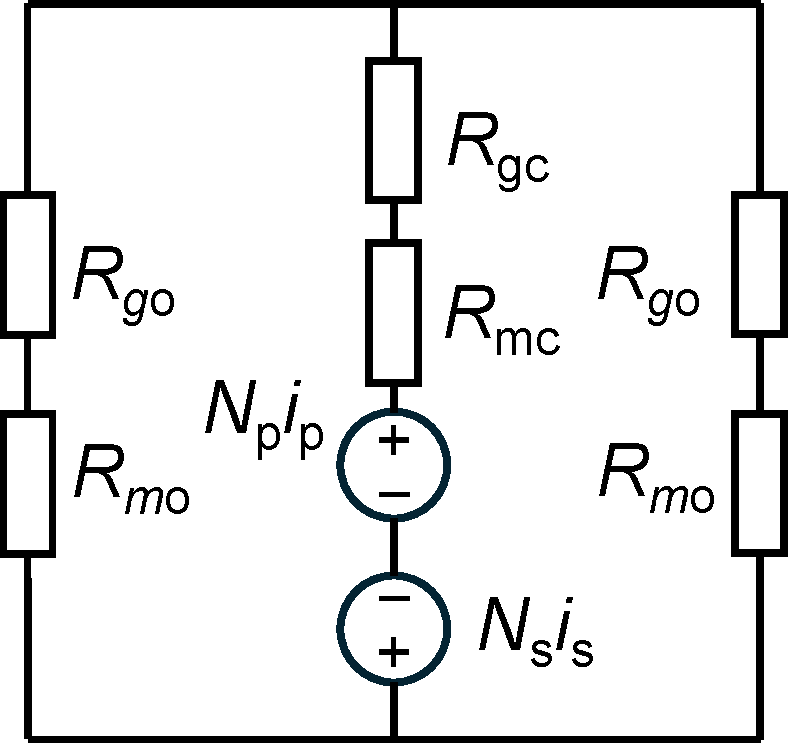
\includegraphics[width=0.35\columnwidth]{figures_chapter3/magnetic_circuit.pdf} 
    
    \caption{Magnetic circuit considered for the proposed transformer in this study.} \label{fig:mag}
\end{figure}

An air gap ($l_g$) is deliberately introduced into the core legs to increase the total reluctance, thereby preventing magnetic saturation under high current excitation and also at operating temperature. Since the transformer is expected to have a wide cross-sectional area, and it is important to obtain an accurate magnetizing inductance for the ZVS operation of the converter, the fringing effect is taken into account when obtaining the cross-sectional area $A_\mathrm{core}$ for the transformer. The method described in \cite{muhlethaler2011novel} is utilized to fine-tune $A_\mathrm{core}$.

\subsection{Core Loss Model}
The improved Generalized Steinmetz Equation (iGSE) is used to obtain the core losses and is able to accommodate a variety of excitation waveforms for the transformer \cite{ref14}. The loss density of a transformer is given in Eq. \ref{eq:igse}, and is multiplied to the core volume to obtain the total core loss:
\begin{equation}
P_{\mathrm{v}} = \frac{1}{T} \int_{0}^{T} k_i \left| \frac{dB}{dt} \right|^\alpha (\Delta B)^{\beta-\alpha} \, dt
\label{eq:igse}
\end{equation}
\noindent with $k_i$ defined in Eq. \ref{eq:ki}:
\begin{equation}
k_i = \frac{k}{(2\pi)^{\alpha-1} \int_{0}^{2\pi} |\cos \theta|^\alpha 2^{\beta-\alpha} \, d\theta}
\label{eq:ki}
\end{equation}
\noindent where $B$ represents the flux density in the transformer during operation, $T$ is the switching period, and $k$, $\alpha$ and $\beta$ represent the Steinmetz parameters of the core material obtained from the datasheet.

For a CLLC, the $B_\mathrm{pk}$ and $\Delta B$ is defined in Eq. \ref{eq:Bpk} and \ref{eq:delB} respectively.
\begin{align}
B_{\mathrm{pk}} &= \frac{V_{\mathrm{pri, pk}} \cdot T_\mathrm{s}}{4 \cdot N_\mathrm{p} \cdot A_{\mathrm{core}}}\label{eq:Bpk}\\
\Delta B &= \frac{V_{\mathrm{pri, pk}} \cdot \frac{T_s}{2}}{N_\mathrm{p}\cdot A_{\mathrm{core}}} \label{eq:delB}
\end{align}
where $V_{\mathrm{pri, pk}}$ is the peak primary side voltage,  $T_\mathrm{s}$ is the switching period, $N_\mathrm{p}$ is the number of turns in the primary side, and $A_\mathrm{core}$ is the cross-sectional area of the transformer center leg.

\subsection{Winding Loss Model}
Dowell's model for rectangular windings with a high width ($h_{\mathrm{wire}}$ for the proposed transformer) to thickness ($w_{\mathrm{wire}}$ for the proposed transformer) ratio, is presented in Equation \ref{eq:dowell} \cite{ref15, ref16}. This equation determines the resistance factor $F_{\mathrm{R}}$ for a turn, defined as the ratio of AC resistance to DC resistance:
\begin{equation}
\begin{split}
F_{\mathrm{R}} = \frac{\xi}{2} \Bigg[ &\frac{\sinh \xi + \sin \xi}{\cosh \xi - \cos \xi} + (2m^2 - 1) \frac{\sinh \xi - \sin \xi}{\cosh \xi + \cos \xi} \Bigg]
\end{split}
\label{eq:dowell}
\end{equation}
\noindent where the first and second terms represent the effects due to the proximity and skin effects, respectively. Moreover, $\xi$ and $m$ represent the penetration ratio and $m$-factor respectively. The penetration ratio $\xi$ is defined as $\xi = w_{\mathrm{wire}}/\delta$ for the flatwise-wound transformer. The skin depth $\delta$  at the operating frequency is given by Eq. \ref{eq:skindepth}:
\begin{equation}
\delta = \sqrt{\frac{\rho}{\pi \mu_r \mu_0 f_\mathrm{s}}}
\label{eq:skindepth}
\end{equation}
\noindent where $\rho$ is the resistivity of the conductor material, which is copper for the windings, $\mu_r$ and $\mu_0$ are the relative permeabilities of the conductor and free space respectively, and $f_s$ is the switching frequency.

The $m$-factor represents the total magnetomotive force ($F$) at a certain turn, divided by its change compared to $F$ at the first turn, as described in Eq. \ref{eq:mfactor}:
\begin{equation}
m = \frac{F(h)}{F(h)-F(0)}
\label{eq:mfactor}
\end{equation}
\noindent For a fully-interleaved winding configuration, $m = 1$.
The winding loss is defined as Eq. \ref{eq:loss}:
\begin{equation}
P_{\mathrm{wind}} = I_{\mathrm{wind}}^2 R_{\mathrm{AC, total}}
\label{eq:loss}
\end{equation}

\noindent where $I_{\mathrm{wind}}$ is the rms value of the transformer winding current and $R_{\mathrm{AC, total}}$ is the total AC Resistance of all turns. For the circuit used in this study, it is approximated to be the input power $P_{\mathrm{in}}$ divided by the input voltage $V_{\mathrm{in}}$ because the transformer is designed on a 1:1 turns ratio.  

\section{Design Considerations}
\par The proposed transformer is designed for a 1kW bidirectional CLLC resonant converter, as had been described in Chapter 2. The detailed specifications are summarized in Table \ref{tab:specs}.
\begin{table}[h]
    \caption{CLLC Converter Specifications}
    \centering
        \begin{tabular}{cccc}
            \hline
            \textbf{Parameter} & \textbf{Symbol} & \textbf{Value} & \textbf{Unit} \\
            \hline \hline
            Input Voltage & $V_{\mathrm{in}}$ & 100 & V \\
            Switching Frequency & $f_{\mathrm{s}}$ & 28.5 & kHz \\
            Primary Side Current & $I_{\mathrm{p, rms}}$ & 10 & A \\
            Transformer Turns Ratio & $n$ & 1 : 1& - \\
            Output Power & $P_{\mathrm{O}}$ & 1 & kW \\
            \hline
        \end{tabular}%
    \label{tab:specs}
\end{table}

\subsection{Design Method}
The design flow for the proposed transformer is depicted in Figure~\ref{fig:design_flow}. Initially, the circuit parameters and constraints are determined. A geometric model is then selected to ensure the transformer aspect ratio falls within the feasible range of 0.25 $\sim$ 0.75. Analytical calculations are then performed to verify that the core and winding losses are balanced ($P_{\mathrm{core}}/P_{\mathrm{wind}} \approx \text{0.50} - \text{1.50}$). The values provided here for the loss balance are just estimates and should be further fine-tuned or explored. Once these conditions are met, the model undergoes thermal and electromagnetic simulation. Ultimately, the design is accepted only if it satisfies the thermal limit of less than 100$^\circ$C peak temperature and maintains ZVS capability.

\begin{figure}[htbp]
    \centerline{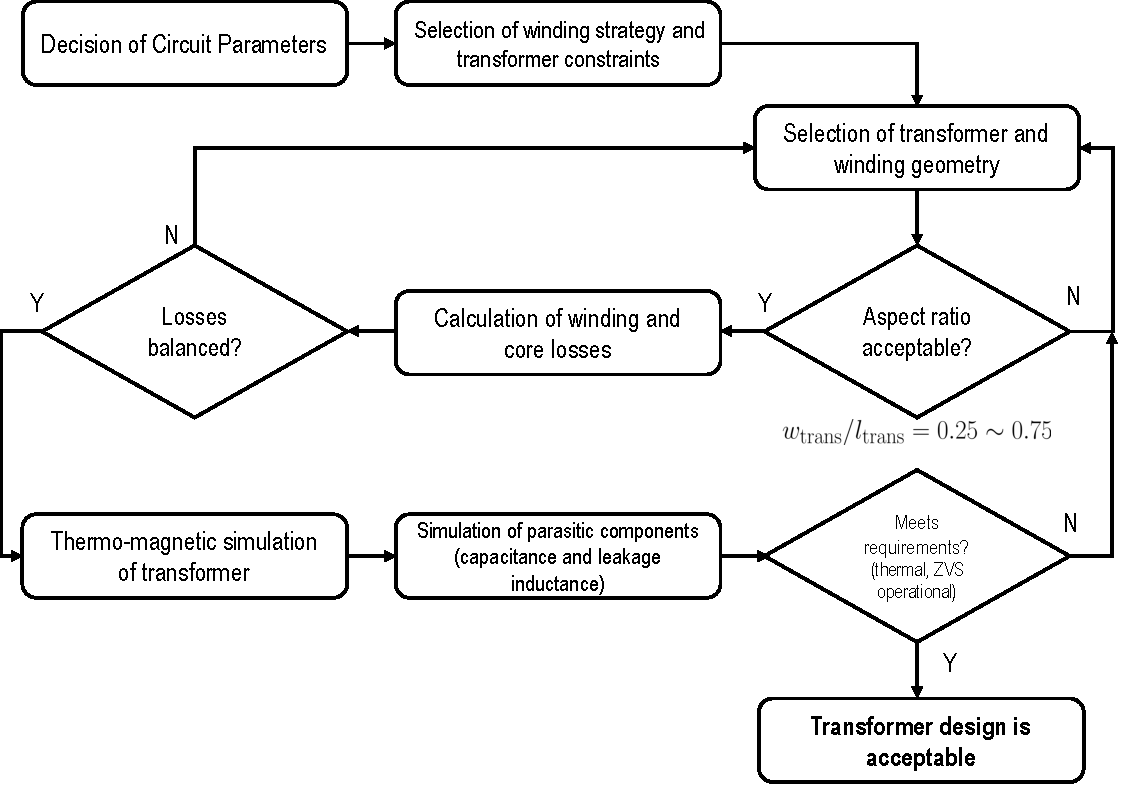
\includegraphics[width=\columnwidth]{figures_chapter3/designflow.pdf}}
    \caption{Design flow for the proposed transformer.}
    \label{fig:design_flow}
\end{figure}

\subsection{Magnetizing and Leakage Inductance}
As discussed in Section \ref{ref:FHA}, to ensure ZVS, the magnetizing inductance is constrained by Eq. \ref{eq:Lm_constraint}

\begin{equation}
L_m \le \frac{t_\mathrm{d}}{16 C_{\mathrm{oss}} f_{\mathrm{r}}}
\label{eq:Lm_constraint}
\end{equation}

\noindent where $t_{\mathrm{d}}$ is defined as the dead time, $C_{\mathrm{oss}}$ is the parasitic output capacitance of the switches, and $f_\mathrm{r}$ is the resonant frequency of the circuit.

\subsection{Number of Turns, Wire Thickness, and Inter-winding Distance}
\par As detailed in Section \ref{section:heat_dissipation}, maximizing the window fill factor is a primary design objective. Since a custom core is utilized to optimize the thermal path, careful selection of the winding geometry is crucial to minimize the overall transformer volume.

The number of turns, wire thickness, and inter-winding distance present trade-offs regarding the transformer volume and total losses. These trade-offs are examined to optimize the geometric parameters for high power density. For this comparison, the center leg width is fixed at 10 mm, the current density $J$ at 5 A/mm$^2$, and the magnetizing inductance $L_{\mathrm{m}}$ at 200 $\upmu$H. Moreover, $d_{\mathrm{TIM}}$ and $d_{\mathrm{clear}}$ are set to 1.00 mm each. The design is evaluated assuming a full interleaving configuration, as detailed in the subsequent subsection.

The interwinding distance $d_{\mathrm{inter}}$ is set to 0.10 mm, providing a safety factor of approximately two relative to the breakdown voltage of air (3 kV/mm) at the operating condition. Air was chosen as the insulation for this study, as the specifications do not entail high voltage yet. 

The design space is illustrated in Figure \ref{fig:trans_design}. The analysis reveals that increasing the number of turns significantly decreases the transformer volume, provided the wire width remains narrow. Conversely, increasing the wire width monotonically increases the volume; however, the rate of volume expansion depends on the turn count. Consequently, eight turns was identified as the optimal design point. Furthermore, the turn count, wire width, and spacing must be balanced to maintain a valid transformer aspect ratio.

The sensitivity of the volume and losses to the turn count emphasizes the necessity of minimizing $d_{\mathrm{inter}}$ until a safe breakdown threshold. Finally, $w_{\mathrm{wire}}$ is constrained to less than 2$\delta$ \cite{ref20}. This limit prevents the proximity effect from dominating the current distribution, which would otherwise induce excessive AC losses at the operating frequency. Based on the design space analysis, $w_\mathrm{wire}$ is selected as 0.30 mm. The resulting window area effectively becomes a square. The chosen design will be explained more in the next chapter.



An example of the loss calculation method analytically is provided in Appendix: \nameref{app:model} for the chosen design point $N_\mathrm{p} = 8$ and $w_\mathrm{wire} = 0.30$ mm.

\begin{figure}[t!]
    \centerline{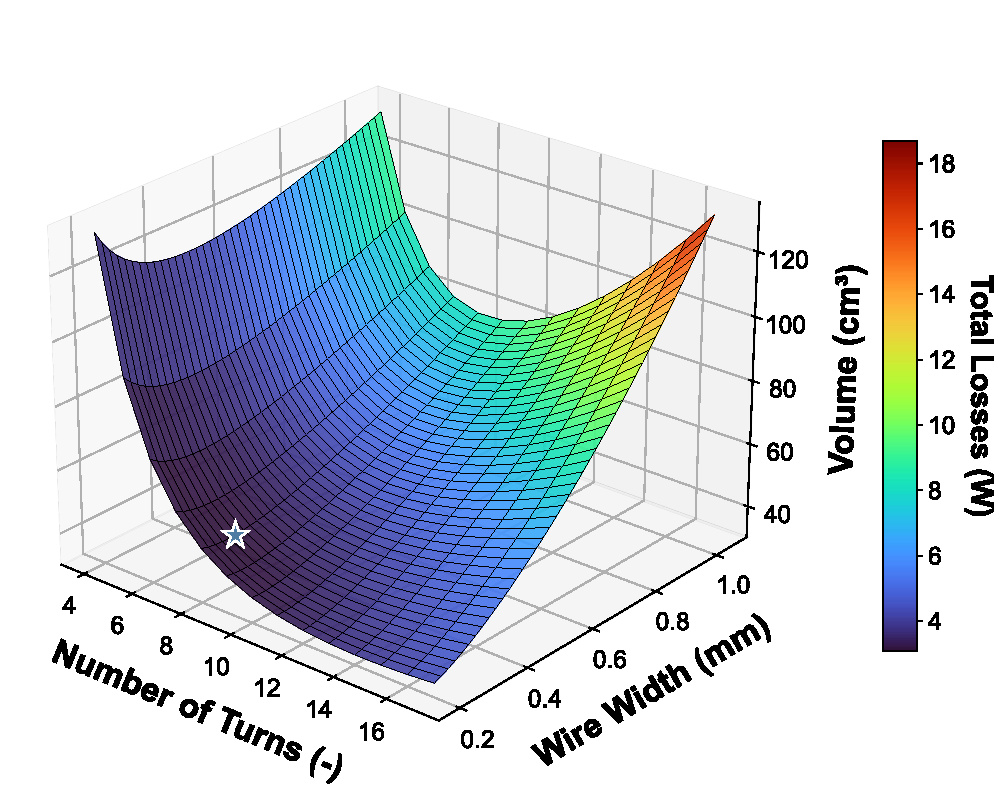
\includegraphics[width=0.8\columnwidth]{figures_chapter3/pareto.pdf}}
    \caption{Trade-off between number of turns and wire width for the flatwise-wound transformer. The selected design is marked as a star.}
    \label{fig:trans_design}
\end{figure}





